\documentclass[11pt]{article}
\usepackage[T1]{fontenc}
\usepackage{lmodern}
\pdfglyphtounicode{parenleftbig}{0028}
\pdfglyphtounicode{parenrightbig}{0029}
\pdfglyphtounicode{parenleftBig}{0028}
\pdfglyphtounicode{parenrightBig}{0029}
\pdfgentounicode=1
\usepackage[margin=1.05in]{geometry}
\usepackage{amsmath,amssymb,amsthm,mathtools}
\usepackage{microtype}
\usepackage{enumitem}
\usepackage{needspace,float}
\usepackage{tikz}
\usetikzlibrary{arrows.meta,positioning,calc}
\usepackage[hidelinks]{hyperref}
\hypersetup{pdftitle={Understanding the second-neighborhood proof},
 pdfauthor={Codex (exposition); OpenAI (source preprint)}, pdfsubject={Oriented graphs and finite relations}}
\pdftrailerid{}
\newtheorem{theorem}{Theorem}[section]
\newtheorem{lemma}[theorem]{Lemma}
\newtheorem{proposition}[theorem]{Proposition}
\newtheorem{corollary}[theorem]{Corollary}
\theoremstyle{remark}
\newtheorem{remark}[theorem]{Remark}
\newcommand{\abs}[1]{\lvert #1\rvert}
\DeclareMathOperator{\rank}{rank}
\DeclareMathOperator{\im}{im}
\newcommand{\R}{\mathbb R}
\title{Understanding the second-neighborhood proof}
\author{Codex exposition of the supplied OpenAI preprint}
\date{November 13, 2026}
\begin{document}
\maketitle
\begin{abstract}
This is an illustrated, expanded exposition of the supplied September 23,
2026 preprint by OpenAI. We explain its counterexample reduction, its
relation-theoretic pruning lemma, and the extremal argument joining them.
The mathematical proof text is retained with additional explanations,
worked examples, and diagrams. The main contribution of this version is
exposition; it is not an independent claim of priority. The accompanying
verification ledger distinguishes mathematical review, finite experiments,
and the scope of the Lean development.
\end{abstract}
\tableofcontents
\section*{How to read this exposition}
\addcontentsline{toc}{section}{How to read this exposition}
The question concerns \emph{distinct vertices}, not the number of paths.
The proof answers a local question about one vertex by introducing sets of
vertices, then sets of ordered pairs, then matrices. Each change of language
has a specific purpose. Write $F(S)=\{y:x\to y\text{ for some }x\in S\}$
and $F^2(S)=F(F(S))$; these are set images with no subtraction.
Keep the following chain in view.
\begin{figure}[ht]
\centering
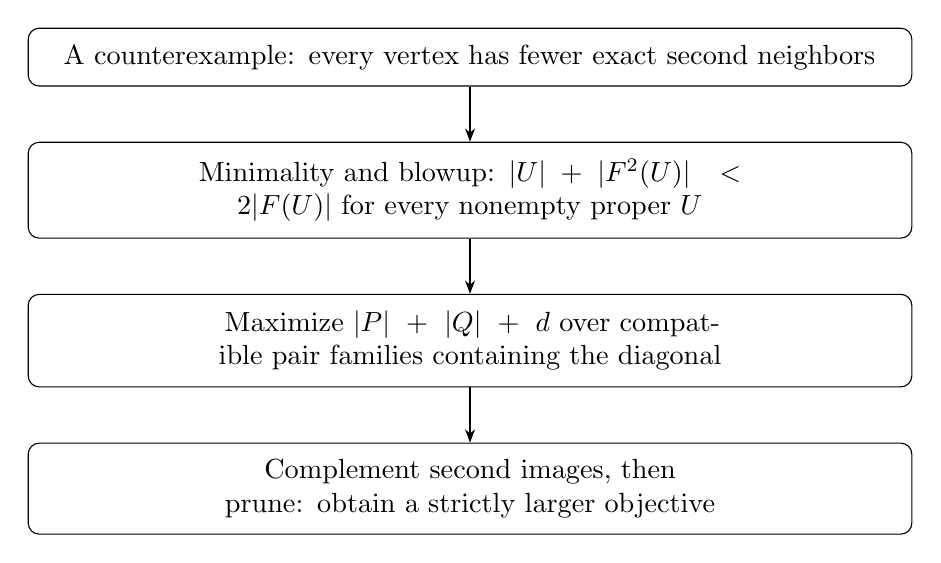
\begin{tikzpicture}[>=Stealth,box/.style={draw,rounded corners,text width=10.8cm,align=center,inner sep=6pt},node distance=7mm]
\node[box] (a) {A counterexample: every vertex has fewer exact second neighbors};
\node[box,below=of a] (b) {Minimality and blowup: $|U|+|F^2(U)|<2|F(U)|$ for every nonempty proper $U$};
\node[box,below=of b] (c) {Maximize $|P|+|Q|+d$ over compatible pair families containing the diagonal};
\node[box,below=of c] (d) {Complement second images, then prune: obtain a strictly larger objective};
\draw[->] (a)--(b);\draw[->] (b)--(c);\draw[->] (c)--(d);
\end{tikzpicture}
\caption{The dependency chain. The last step uses the pruning lemma, which is proved independently for arbitrary finite relations.}
\end{figure}

\paragraph{Choose a reading route.}
For a five-minute overview, follow the dependency figure, the main theorem,
and the accounting diagram in Section~\ref{sec:incompatibility}.
For a longer first reading, follow the two passes below, accepting pruning
before examining its proof. For a complete verification, use the correctness
ledger and the Lean status document alongside the formal statements. These
routes are adapted from the reading levels in the DeepSeep4.1 rewrite.

\paragraph{Check the ambient set as well as the subsets.}
The main theorem, the graph produced by the reduction, and the no-concavity
proposition all require a nonempty vertex set. A universal claim about
nonempty proper subsets says nothing when the ambient set is empty. The
pruning lemma, in contrast, is valid for an empty ambient set too.

\paragraph{A first pass.}
Read the definitions, the two reduction statements, the pruning statement,
and the extremal proof. On this pass accept the pruning lemma as a tool.
Its unusual cost is the key: deletion is charged partly to points uncovered
\emph{after} pruning. Then return to the linear algebra proving that cost.

\paragraph{A close pass.}
In the reduction, check the exact gain/loss identity for $g(T)$ and the
full-support exception in the blowup. In pruning, check which coordinate
moves forward and which backward, and why all generic rank conditions can
hold at once. In the final proof, check that every fiber is proper and the
diagonal survives. These are the places where an innocent change of
convention would invalidate the argument.

\subsection*{A small example that fixes the conventions}
\begin{figure}[ht]
\centering
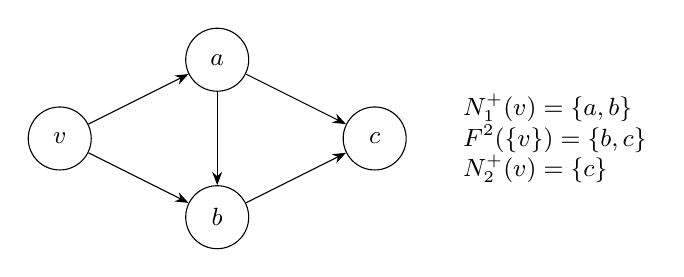
\begin{tikzpicture}[>=Stealth,v/.style={circle,draw,minimum size=8mm},every node/.style={font=\small}]
\node[v] (v) at (0,0) {$v$};\node[v] (a) at (2,1) {$a$};
\node[v] (b) at (2,-1) {$b$};\node[v] (c) at (4,0) {$c$};
\draw[->] (v)--(a);\draw[->] (v)--(b);\draw[->] (a)--(b);
\draw[->] (a)--(c);\draw[->] (b)--(c);
\node[align=left,anchor=west] at (5,0) {$N_1^+(v)=\{a,b\}$\\$F^2(\{v\})=\{b,c\}$\\$N_2^+(v)=\{c\}$};
\end{tikzpicture}
\caption{All arcs in this example are drawn. Two paths reach $c$, but it is counted once. The vertex $b$ is reached in two steps and in one step, so it is excluded from the exact second neighborhood. This graph is not a counterexample: $c$ is a sink.}
\end{figure}
For an arbitrary set $S$, the image $F(S)$ may meet $S$. For example,
on a directed triangle and $S$ equal to the whole vertex set, $F(S)=S$.
Never replace a set-image by its exterior neighborhood without explicitly
subtracting $S$. For a singleton in an oriented graph, $v\notin F^2(\{v\})$
because a return in two steps would require opposite arcs. Thus the source's
formula $N_2^+(v)=F^2(\{v\})\setminus F(\{v\})$ is valid.

\Needspace{13\baselineskip}
\paragraph{Notation dictionary.}
\begin{center}
\begin{tabular}{p{2.5cm}p{9cm}}
$D$, then $G$ & Minimal counterexample, then its tournament blowup.\\
$F$, $F^2$ & Union of out-neighbors; its iterate, with no subtraction.\\
$P,Q$ & Compatible left and right families of ordered pairs.\\
$F_1,F_2$ & Advance the first or second coordinate along an arc.\\
$d$ & Points in neither coordinate image of the current pair.\\
$\mathcal R,\mathcal C$ & Prospective families before pruning.\\
$H,Z$ & The two opposite intermediate corners of conflicts.\\
$\Phi$, $\Phi^{p,i}$ & Matrices in the pruning proof; $D$ remains a graph.\\
$L,N,B,A$ & Linear maps in the commuting square used only in pruning.
\end{tabular}
\end{center}
The symbols $I,E,T,Q,C$ in the subset-deficit proof are local to that proof;
in particular its set $Q$ is unrelated to the later pair family $Q$.

\section{Introduction}\label{sec:introduction}

An \emph{oriented graph} is a finite directed graph with no loops, no multiple
arcs, and no pair of opposite arcs.  Its underlying undirected graph need
not be complete or connected.  For a vertex \(v\), write
\[
 N_1^+(v)=\{u:v\to u\},\qquad
 N_2^+(v)=\{w\notin\{v\}\cup N_1^+(v):
                 \text{ there is a vertex }u\text{ with }v\to u\to w\}.
\]
Thus \(N_2^+(v)\) consists of the vertices at directed distance exactly two
from \(v\).  Each vertex is counted once, regardless of the number of paths
reaching it.  Seymour's second neighborhood conjecture asserts that some
vertex satisfies \(\abs{N_1^+(v)}\leq\abs{N_2^+(v)}\).

\begin{theorem}\label{thm:main}
Every nonempty finite oriented graph has a vertex \(v\) such that
\[
 \abs{N_1^+(v)}\leq \abs{N_2^+(v)}.
\]
\end{theorem}

The supplied preprint presents Theorem~\ref{thm:main} as a resolution of the conjecture, without a
connectivity or degree hypothesis.  In particular, a sink already satisfies
the conclusion.  The conjecture is a basic comparison between the first two
out-neighborhoods: removing vertices already reached in one step is essential
to its assertion.

The theorem also gives the established vertex- and arc-weighted forms of
the conjecture through Seacrest's equivalences~\cite{Seacrest2015}.
The vertex-weighted conclusions have two different quantifier orders:
for every nonnegative weighting there is a suitable vertex, and there is
a weighting of total mass one for which every vertex is suitable.
Section~\ref{sec:weighted-consequences} states these forms precisely.
Section~\ref{sec:directed-cycle-consequences} records consequences for
short directed cycles.  In particular, a graph with minimum in- and
outdegree at least one third of its order contains a directed triangle.

Our proof builds on the minimal-counterexample and graph-product
methods of Brantner, Brockman, Kay and
Snively~\cite{BrantnerBrockmanKaySnively2009} and on Seacrest's
subset perspective~\cite{Seacrest2019}.
We adapt the edge-deletion idea in the proof of Seacrest's Lemma~4 to
obtain the stronger subset inequality needed here, and give that argument
in full.  The exact set-image convention and inequality are stated below.
The main additional ingredient is a pruning bound for arbitrary finite
binary relations.  Its deletion cost depends on the points left uncovered
after pruning; this dependence makes the final extremal argument possible.

\paragraph{Proof strategy: the three bridges.}
For a digraph \(D\) and a set \(S\) of its vertices, define
\[
 F_D(S)=\{y:\text{ there is }x\in S\text{ with }x\to y\},
 \qquad F_D^2(S)=F_D(F_D(S)).
\]
The operator \(F_D\) does not subtract \(S\).  In an oriented graph there is
no directed walk of length two from a vertex to itself, and hence
\(N_2^+(v)=F_D^2(\{v\})\setminus F_D(\{v\})\).

We first suppose that a counterexample exists and choose one with minimum
order and then minimum number of arcs.  Deleting carefully chosen arcs
shows that every nonempty proper vertex set \(S\) satisfies
\[
 \abs{F_D^2(S)\setminus F_D(S)}
 <
 \abs{F_D(S)\setminus S}.
\]
Replacing each vertex by a sufficiently large transitive tournament turns
this into a strict inequality
\begin{equation}\label{eq:overview-concavity}
 \abs{U}+\abs{F_G^2(U)}<2\abs{F_G(U)}
\end{equation}
for every nonempty proper subset \(U\) of the new oriented graph \(G\).
Every vertex of \(G\) has positive indegree.  These reductions are proved in
Section~\ref{sec:reduction}.

The obstruction to~\eqref{eq:overview-concavity} is an extremal argument
on two families of ordered pairs in $V(G)\times V(G)$.  A coordinate image
advances that coordinate along an arc of $G$ and leaves the other coordinate
fixed.  The families are compatible when the first-coordinate image of the left family and the
second-coordinate image of the right family are disjoint.  A point in
neither image is called uncovered.  Require both families to contain the
diagonal, write $M$ for their combined size and $d$ for the number of
uncovered points, and maximize $M+d$ over all such compatible pairs.
The columns of the left family and the rows of the right family are
nonempty proper vertex sets, so
\eqref{eq:overview-concavity} applies to each of them.  Taking complements
of the second iterated images then produces prospective families with
combined size greater than $M+2d$.

These families may conflict, but their diagonal members are still present
and conflict-free.  The pruning lemma in
Section~\ref{sec:pruning}, valid for every finite binary relation,
restores compatibility and preserves their diagonal members.
In this application its two deletion-cost terms are at most $d$ and $d'$,
where $d'$ is the number of points left uncovered by the retained families.
Thus at most $d+d'$ members are deleted, and the new extremal objective is
strictly greater than
\[
 M+2d-(d+d')+d'=M+d.
\]
Section~\ref{sec:incompatibility} proves these bounds and obtains the
contradiction.  This is why the pruning lemma must charge part of its
cost to the points left uncovered after deletion.

The pruning proof bounds a matching in an augmented bipartite graph.
Changing the two coordinates of a pair in opposite orders factors the
same matrix through two different index sets attached to a conflict.
A simultaneous maximum-rank choice of the entries makes the kernels of
these maps control the matching size.  The full argument is independent
of the orientation assumption and is given in Section~\ref{sec:pruning}.

\section{From a counterexample to a strict subset inequality}
\label{sec:reduction}

We first convert a hypothetical counterexample into a graph whose first
image is larger than the average of a set and its second image.  Throughout
this section, $F=F_D$ denotes the ordinary union of the out-neighborhoods
in a specified base graph $D$; in particular, $F(S)$ need not be disjoint
from $S$.

\begin{proposition}[Counterexample reduction]
\label{prop:counterexample-reduction}
If Theorem~\ref{thm:main} has a counterexample, then there is a finite
nonempty oriented graph $G$ in which every vertex has positive indegree
and
\begin{equation}
\label{eq:strict-subset-growth}
  \abs{U}+\abs{F_G^2(U)}<2\abs{F_G(U)}
  \qquad\text{for every }\varnothing\ne U\subsetneq V(G).
\end{equation}
\end{proposition}

There are two steps.  Minimality first gives a strict deficit for subsets
of a counterexample.  Replacing each vertex by a sufficiently large
transitive tournament then turns that deficit into
\eqref{eq:strict-subset-growth}.

The arc-deletion argument below adapts the proof idea of
\cite[Lemma~4]{Seacrest2019}.  Specializing Seacrest's parameter $\lambda$
to $1$, his statement gives
$\abs{F^2(S)\setminus F(S)}<\abs{F(S)}$ in an edge-minimal
counterexample when $F(S)$ is nonempty.  Lemma~\ref{lem:subset-deficit}
replaces this right-hand bound by $\abs{F(S)\setminus S}$ for nonempty
proper $S$, under the stronger choice of minimum order and then minimum
arc count.  We prove this strengthened form in full.


\paragraph{Why delete arcs?}
Vertex minimality gives strong connectivity. Arc minimality supplies a good
vertex whenever at least one arc is removed. The useful deletion depends on
a set $T$ of already processed exterior neighbors. Its witness $v$ identifies
a nonempty batch $Q$ of new vertices. The potential $g(T)$ measures the
unprocessed image outside $I\cup T$, not all of $F(T)$. Its increment is
smaller than the batch size, so these local inequalities telescope.
\begin{figure}[ht]\centering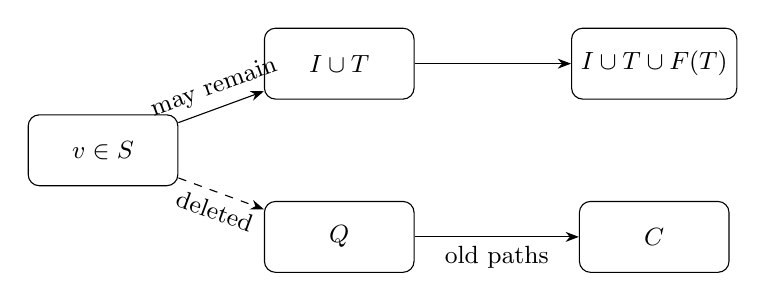
\begin{tikzpicture}[>=Stealth,every node/.style={font=\small},box/.style={draw,rounded corners,minimum width=19mm,minimum height=9mm}]
\node[box] (v) at (0,0) {$v\in S$};
\node[box] (t) at (3,1.1) {$I\cup T$};
\node[box] (q) at (3,-1.1) {$Q$};
\node[box] (f) at (7,1.1) {$I\cup T\cup F(T)$};
\node[box] (c) at (7,-1.1) {$C$};
\draw[->] (v)--node[above,sloped] {may remain} (t);
\draw[->,dashed] (v)--node[below,sloped] {deleted} (q);
\draw[->] (t)--(f);\draw[->] (q)--node[below] {old paths} (c);
\end{tikzpicture}

\caption{Schematic for a deletion step. The dashed arcs from $v$ to $Q$ are removed. Every surviving two-step endpoint lies in the top-right set. The set $C$ consists of old endpoints through $Q$ outside that set and outside $Q$, so all of $C$ is lost. Other arcs are unspecified.}
\end{figure}

\begin{lemma}[Subset deficit]
\label{lem:subset-deficit}
Let $D$ be a finite nonempty oriented graph such that
$\abs{N_1^+(v)}>\abs{N_2^+(v)}$ for every $v\in V(D)$.
Choose $D$ with minimum order and, subject to that, minimum number of
arcs among all graphs with this property.  Then $D$ is strongly connected,
every vertex has positive indegree, and
\begin{equation}
\label{eq:subset-deficit}
  \abs{F^2(S)\setminus F(S)}<\abs{F(S)\setminus S}
  \qquad\text{for every }\varnothing\ne S\subsetneq V(D).
\end{equation}
\end{lemma}

\begin{proof}
A sink satisfies the second-neighborhood inequality, so $D$ has no sink
and has more than one vertex.  If $D$ were not strongly connected, take
a strongly connected component with no outgoing arc to another component.
All first and second out-neighborhoods of its vertices lie in that
component.  Its induced graph would therefore be a smaller counterexample,
contrary to the choice of $D$.  Thus $D$ is strongly connected, and every
vertex has an in-neighbor.

Fix a nonempty proper subset $S$ and put
\[
  I=F(S)\cap S,\qquad E=F(S)\setminus S,
  \qquad g(T)=\abs{F(T)\setminus(I\cup T)}\quad(T\subseteq E).
\]
Strong connectivity gives $E\ne\varnothing$.  We will enlarge $T$ from
$\varnothing$ to $E$ so that the increase in $g(T)$ is strictly smaller
than the number of newly adjoined vertices at every step.

For $T\subsetneq E$, let $D_T$ be obtained from the original graph $D$
by deleting all arcs from $S$ to $E\setminus T$.  Since every vertex of
$E\setminus T$ receives an arc from $S$, at least one arc is deleted.
Minimality of the number of arcs gives a vertex $v$ satisfying
$\abs{N_{1,D_T}^+(v)}\le\abs{N_{2,D_T}^+(v)}$.
If $v$ had lost no first out-neighbor, deleting arcs could only shrink
its exact second out-neighborhood, so it would still violate this
inequality.  Consequently $v\in S$, and the set
\[
  Q=F(\{v\})\cap(E\setminus T)
\]
is nonempty.  It is exactly the set of first out-neighbors that $v$ loses.
The original first out-neighborhood of $v$ is contained in $I\cup T\cup Q$,
and the remaining first out-neighbors lie in $I\cup T$.

We compare the exact second out-neighborhoods before and after deletion.
A two-step path from $v$ in $D_T$ through a vertex of $I\subseteq S$
ends in $I\cup T$, since all arcs from $S$ to $E\setminus T$ were
deleted.  A path through a vertex of $T$ ends in $F(T)$.  Thus
\begin{equation}
\label{eq:deleted-path-endpoints}
  F_{D_T}^2(\{v\})\subseteq I\cup T\cup F(T).
\end{equation}
Every newly counted exact second out-neighbor must have been a first
out-neighbor in $D$: deletion creates no paths, and $v$ itself is never
an exact second out-neighbor.  Such a vertex lies in $Q$, and
\eqref{eq:deleted-path-endpoints}, together with
$Q\cap(I\cup T)=\varnothing$, places it in $Q\cap F(T)$.

On the other hand, define
\[
  C=F(Q)\setminus\bigl(I\cup T\cup Q\cup F(T)\bigr).
\]
Every vertex of $C$ was reached from $v$ in two steps through $Q$, and
none was a first out-neighbor.  Also $v\notin F(Q)$: an arc from a
vertex of $Q$ back to $v$ would oppose the arc from $v$ to that vertex.
Hence $C\subseteq N_{2,D}^+(v)$.  By
\eqref{eq:deleted-path-endpoints}, no vertex of $C$ remains reachable
in two steps in $D_T$.

Write $d_1=\abs{N_{1,D}^+(v)}$ and
$d_2=\abs{N_{2,D}^+(v)}$.  The gains and losses just identified imply
\[
  d_1-\abs{Q}
  \le \abs{N_{2,D_T}^+(v)}
  \le d_2-\abs{C}+\abs{Q\cap F(T)}.
\]
The change in $g$ is exact: adjoining $Q$ removes the points
$Q\cap F(T)$ from the previously counted image and adds precisely $C$.
Since $d_2<d_1$, it follows that
\begin{equation}
\label{eq:deficit-increment}
  g(T\cup Q)-g(T)
  =\abs{C}-\abs{Q\cap F(T)}
  \le \abs{Q}+d_2-d_1
  <\abs{Q}.
\end{equation}

Starting with $T=\varnothing$, repeat this step until $T=E$.
Each deletion is performed afresh on the original $D$, so the same
minimality argument applies at every step.  Each $Q$ is a nonempty
subset of the part of $E$ not yet adjoined; hence the process terminates.
Summing \eqref{eq:deficit-increment} and using $g(\varnothing)=0$
gives $g(E)<\abs{E}$.  Finally,
$F(S)=I\cup E$ and $F(I)\subseteq F(S)$, so
\[
  F^2(S)\setminus F(S)
  =\bigl(F(I)\cup F(E)\bigr)\setminus(I\cup E)
  =F(E)\setminus(I\cup E).
\]
Its cardinality is $g(E)$, proving \eqref{eq:subset-deficit}.
\end{proof}

We next amplify the integer deficit in \eqref{eq:subset-deficit}.
Each unit of the base deficit contributes the entire block size; the
remaining internal contribution costs at most one unit per base vertex.
The construction below is the lexicographic product $D[T_m]$, where $T_m$
is a transitive tournament.  The same graph-product construction appears
in \cite[Theorem~4.3]{BrantnerBrockmanKaySnively2009}; here we need an
estimate for every nonempty proper subset, rather than only for individual
vertices.


\begin{figure}[ht]\centering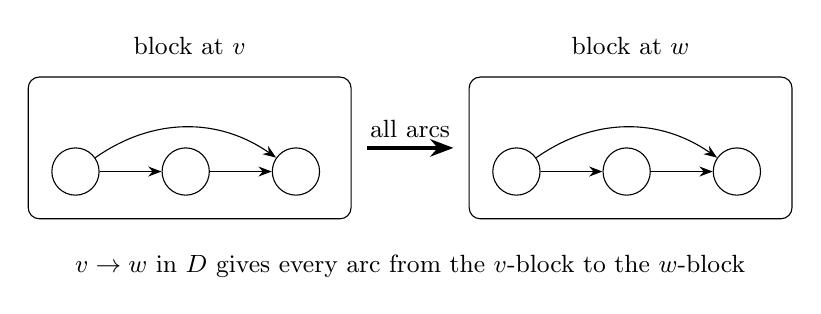
\begin{tikzpicture}[>=Stealth,every node/.style={font=\small},v/.style={circle,draw,minimum size=6mm,inner sep=1pt}]
\draw[rounded corners] (-.6,-.6) rectangle (3.5,1.2);
\draw[rounded corners] (5,-.6) rectangle (9.1,1.2);
\node at (1.45,1.6) {block at $v$};\node at (7.05,1.6) {block at $w$};
\foreach \x/\name in {0/a,1.4/b,2.8/c} {\node[v] (\name) at (\x,0) {};}
\foreach \x/\name in {5.6/d,7/e,8.4/f} {\node[v] (\name) at (\x,0) {};}
\draw[->] (a)--(b);\draw[->] (b)--(c);\draw[->] (a) to[bend left=35] (c);
\draw[->] (d)--(e);\draw[->] (e)--(f);\draw[->] (d) to[bend left=35] (f);
\draw[->,very thick] (3.7,.3)--node[above] {all arcs} (4.8,.3);
\node at (4.25,-1.2) {$v\to w$ in $D$ gives every arc from the $v$-block to the $w$-block};
\end{tikzpicture}

\caption{The blowup, illustrated with three vertices per block. The actual proof uses $m>n$. The thick arrow abbreviates a complete directed bipartite graph, not a single arc. Inside each block all arcs point in the label order.}
\end{figure}
\paragraph{What the amplification buys.}
Write $\delta(S)=|F^2(S)\setminus F(S)|-|F(S)\setminus S|$.
The previous lemma says $\delta(S)\le-1$ for proper nonempty $S$.
In the blowup we will show that the target expression is at most
$m\delta(S)+n$. Choosing $m>n$ makes this negative. This reasoning does not
apply to full support $S=V(D)$; that case has a separate, simpler proof.
For example, in a block of size five, $T=\{2,4\}$ gives
$f(T)=\{3,4,5\}$ and $f^2(T)=\{4,5\}$, so
$|T|-2|f(T)|+|f^2(T)|=-2$. The uniform upper bound is $1$, attained when
$T=\{5\}$. Thus sparse selections and terminal vertices are included.

\begin{lemma}[Transitive-tournament blowup]
\label{lem:blowup}
Let $D$ be an oriented graph on $n\ge1$ vertices, all of positive
indegree, satisfying \eqref{eq:subset-deficit} for every nonempty proper
subset of $V(D)$.  For an integer $m>n$, replace each vertex by a
transitive tournament on $m$ vertices.  For every arc $v\to w$ of $D$,
put all arcs from the block at $v$ to the block at $w$, and put no other
arcs between distinct blocks.  The resulting graph $G$ is oriented,
all its indegrees are positive, and it satisfies
\eqref{eq:strict-subset-growth}.
\end{lemma}

\begin{proof}
Label the vertices within each block by $1,\ldots,m$, with arcs from
smaller to larger labels.  Let $f$ be the image operator within this
transitive tournament.  For a nonempty set $T$ of labels with least
element $a$, we have $f(T)=\{a+1,\ldots,m\}$.  Thus
\begin{equation}
\label{eq:internal-block-bound}
  \abs{T}-\abs{f(T)}\le1,\qquad
  f^2(T)\subseteq f(T),\qquad
  \abs{T}-2\abs{f(T)}+\abs{f^2(T)}\le1.
\end{equation}
The construction produces an oriented graph.  Every vertex receives
arcs from an incoming base block, so all indegrees in $G$ are positive.
Call an arc external if it joins distinct blocks, and internal otherwise.

Fix $\varnothing\ne U\subsetneq V(G)$.  Write $T_v$ for the labels
selected by $U$ in the block at $v$, and define its support and a set
of base vertices by
\[
  S=\{v\in V(D):T_v\ne\varnothing\},\qquad
  H_0=F(S)\cup F^2(S).
\]
Every block indexed by $F(S)$ is filled by $F_G(U)$.  In each remaining
block the first image consists exactly of $f(T_v)$, so
\[
  \abs{F_G(U)}=m\abs{F(S)}
     +\sum_{v\in S\setminus F(S)}\abs{f(T_v)}.
\]
A two-step path using two external arcs ends in an $F^2(S)$-block.
One using exactly one external arc ends in an $F(S)$-block, regardless
of the order of its internal and external steps.  Paths using only
internal arcs contribute $f^2(T_v)$.  Therefore
\[
  \abs{F_G^2(U)}\le m\abs{H_0}
     +\sum_{v\in S\setminus H_0}\abs{f^2(T_v)}.
\]
Combining these estimates gives the sharper bound
\begin{align}
\label{eq:blowup-sharp}
  \abs{U}-2\abs{F_G(U)}+\abs{F_G^2(U)}
  &\le m\bigl(\abs{H_0}-2\abs{F(S)}\bigr)
       +\sum_{v\in S}\abs{T_v} \notag\\
  &\quad -2\sum_{v\in S\setminus F(S)}\abs{f(T_v)}
       +\sum_{v\in S\setminus H_0}\abs{f^2(T_v)}.
\end{align}
Since $F(S)\subseteq H_0$, extending the last sum to
$S\setminus F(S)$ only adds nonnegative terms.  This may count internal
second images in blocks already bounded by a full block in
\eqref{eq:blowup-sharp}; it remains a valid upper bound.  Now use
$\abs{T_v}\le m$ on $S\cap F(S)$ and
\eqref{eq:internal-block-bound} on $S\setminus F(S)$ to obtain
\begin{align*}
  \abs{U}-2\abs{F_G(U)}+\abs{F_G^2(U)}
  &\le m\bigl(\abs{H_0}-2\abs{F(S)}
                    +\abs{S\cap F(S)}\bigr)
       +\abs{S\setminus F(S)}\\
  &\le m\bigl(\abs{F^2(S)\setminus F(S)}
                    -\abs{F(S)\setminus S}\bigr)+n.
\end{align*}
If $S\subsetneq V(D)$, the parenthesized difference is an integer
strictly less than zero by \eqref{eq:subset-deficit}.  The last bound
is consequently at most $-m+n<0$.

It remains to consider $S=V(D)$, for which the subset-deficit hypothesis
does not apply.  Positive indegrees in $D$ give $F(S)=V(D)$, so
$F_G(U)=V(G)$.  Positive indegrees in $G$ then give
$F_G^2(U)=V(G)$ as well.  In this case
\[
  \abs{U}-2\abs{F_G(U)}+\abs{F_G^2(U)}
  =\abs{U}-\abs{V(G)}<0,
\]
because $U$ is proper.  This proves the required inequality for every
allowed $U$.
\end{proof}

\begin{proof}[Proof of Proposition~\ref{prop:counterexample-reduction}]
Choose a counterexample of minimum order and then minimum number of
arcs.  Lemma~\ref{lem:subset-deficit} supplies positive indegrees and
the subset deficit, so Lemma~\ref{lem:blowup}, with any integer
$m>\abs{V(D)}$, supplies the required graph $G$.
\end{proof}

\section{Pruning two families of pairs}\label{sec:pruning}

We now prove a deletion bound for two families of ordered pairs.  The bound
charges the deleted members to two sets of pairs: one determined by the
original conflicts, and the other consisting of points left uncovered after
deletion.  This dependence on the surviving families will be essential in
Section~\ref{sec:incompatibility}.  The result holds for every finite binary
relation; no orientation assumption is needed.


\paragraph{Read the conclusion before the proof.}
An ordinary conflict cover would only tell us how many members must go.
Here we need a cover whose cost improves whenever the kept families cover
more points of $Z$. Put $q=|Z\setminus(F_1\mathcal R'\cup F_2\mathcal C')|$.
The desired inequality is ``deletions $\le |H|+q$''. The term $q$ depends
on the output, so one cannot choose it in advance. The augmentation by two
copies of $Z$ converts output coverage into a discount on deletions.

\begin{lemma}[Pruning]\label{lem:pruning}
Let $X$ be a finite set with a binary relation denoted by $\to$, and let
$\mathcal R,\mathcal C\subseteq X\times X$ be two families, regarded as
separate copies even when their coordinates agree.  Say that
$(p,j)\in\mathcal R$ and $(i,s)\in\mathcal C$ \emph{conflict} if
\[
 p\to i\qquad\text{and}\qquad s\to j.
\]
Define
\begin{align*}
 Z&=\{(i,j):\text{some }(p,j)\in\mathcal R
       \text{ conflicts with some }(i,s)\in\mathcal C\},\\
 H&=\{(p,s):\text{some }(p,j)\in\mathcal R
       \text{ conflicts with some }(i,s)\in\mathcal C\}.
\end{align*}
A point $(i,j)$ is \emph{covered} by a member $(p,j)\in\mathcal R$ when
$p\to i$, and by a member $(i,s)\in\mathcal C$ when $s\to j$.
These are the only ways a member covers a point.

There are subfamilies $\mathcal R'\subseteq\mathcal R$ and
$\mathcal C'\subseteq\mathcal C$ with no conflicts between them such that
every initially conflict-free member is retained and
\begin{equation}\label{eq:pruning-bound}
 \abs{\mathcal R\setminus\mathcal R'}+
 \abs{\mathcal C\setminus\mathcal C'}
 \leq \abs H+
 \abs{\{z\in Z:z\text{ is covered by no member of }
                    \mathcal R'\cup\mathcal C'\}}.
\end{equation}
The two sides are counted separately throughout.
\end{lemma}

\subsection*{A worked example: extra deletion can be necessary}
Let $X=\{0,1,2\}$ and let the only arrows be $0\to1$ and $0\to2$.
Take $\mathcal R=\{(0,1),(0,2)\}$ and
$\mathcal C=\{(1,0),(2,0)\}$. Every left member conflicts with every
right member. The corner sets are
\[
H=\{(0,0)\},\qquad Z=\{1,2\}\times\{1,2\}.
\]
\begin{figure}[H]\centering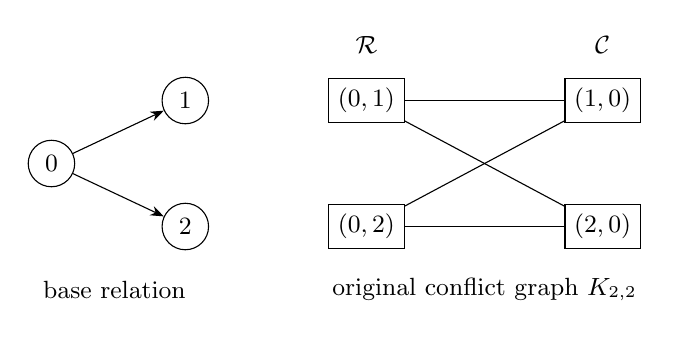
\begin{tikzpicture}[>=Stealth,every node/.style={font=\small}]
\node[draw,circle] (x) at (0,0) {$0$};
\node[draw,circle] (y) at (1.7,.8) {$1$};
\node[draw,circle] (z) at (1.7,-.8) {$2$};
\draw[->] (x)--(y);\draw[->] (x)--(z);
\node at (.8,-1.6) {base relation};
\node[draw] (r1) at (4,.8) {$(0,1)$};
\node[draw] (r2) at (4,-.8) {$(0,2)$};
\node[draw] (c1) at (7,.8) {$(1,0)$};
\node[draw] (c2) at (7,-.8) {$(2,0)$};
\draw (r1)--(c1);\draw (r1)--(c2);\draw (r2)--(c1);\draw (r2)--(c2);
\node at (4,1.5) {$\mathcal R$};\node at (7,1.5) {$\mathcal C$};
\node at (5.5,-1.6) {original conflict graph $K_{2,2}$};
\end{tikzpicture}

\caption{All arrows of the base relation and all four original conflicts are shown. The crossed lines in the conflict graph do not introduce a vertex at their intersection. The augmented graph additionally has two copies of each of the four points of $Z$.}
\end{figure}
Deleting either entire family is an ordinary minimum conflict cover of
size two. The other family then covers every point of $Z$, so $q=0$.
Such a choice fails the desired bound $2\le |H|+q=1$.
Instead, keep just $(0,1)$ on the left and nothing on the right.
There are three deletions. The kept member covers $(1,1)$ and $(2,1)$;
the two points in the other column are uncovered. Thus $q=2$ and
$3=|H|+q$. The lemma promises a suitable pruning, not that every smallest
cover of the original conflict graph works. This example explains why the
augmented graph is needed.

\paragraph{The two corner sets cannot be interchanged.}
The previous example has $|H|=1$ and $|Z|=4$. For the reverse imbalance,
let the only arcs be $0\to2$ and $1\to2$, and take
\[
\mathcal R=\{(0,2),(1,2)\},\qquad
\mathcal C=\{(2,0),(2,1)\}.
\]
Now $H=\{0,1\}\times\{0,1\}$, while $Z=\{(2,2)\}$.
Every left member conflicts with every right member, and every member
covers the sole point of $Z$. Any conflict-free pruning with a survivor
therefore has $q=0$ and at least two deletions. With no survivors it has
$q=1$ and four deletions. Thus replacing $|H|+q$ by $|Z|+q$ would fail
in both cases, even for this acyclic oriented graph. The correct bound
allows keeping all of $\mathcal R$ and deleting $\mathcal C$, at cost
$2\le |H|=4$. In words, $Z$ records where the original images meet;
$H$ records the opposite corners charged by the lemma.
\begin{figure}[H]\centering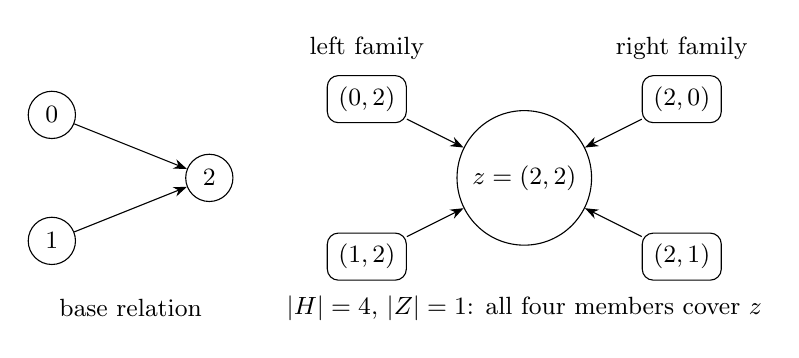
\begin{tikzpicture}[>=Stealth,every node/.style={font=\small},v/.style={circle,draw,minimum size=6mm},member/.style={draw,rounded corners,inner sep=4pt}]
\node[v] (a) at (0,.8) {$0$};\node[v] (b) at (0,-.8) {$1$};\node[v] (c) at (2,0) {$2$};
\draw[->] (a)--(c);\draw[->] (b)--(c);
\node at (1,-1.65) {base relation};
\node[member] (l1) at (4,1) {$(0,2)$};\node[member] (l2) at (4,-1) {$(1,2)$};
\node[member] (r1) at (8,1) {$(2,0)$};\node[member] (r2) at (8,-1) {$(2,1)$};
\node[draw,circle,inner sep=4pt] (z) at (6,0) {$z=(2,2)$};
\draw[->] (l1)--(z);\draw[->] (l2)--(z);\draw[->] (r1)--(z);\draw[->] (r2)--(z);
\node at (4,1.65) {left family};\node at (8,1.65) {right family};
\node at (6,-1.65) {$|H|=4$, $|Z|=1$: all four members cover $z$};
\end{tikzpicture}

\caption{The reverse fork gives a four-member counterexample to the incorrect $|Z|+q$ bound. The right-hand incidence graph shows coverage links, not graph arcs or coordinate-grid positions. Every left--right pair conflicts. The correctly stated pruning lemma uses $|H|+q$.}
\end{figure}

The proof will bound a matching in an augmented bipartite graph by using
matrix ranks.  We first record the elementary rank fact that makes the
argument work.  For finite index sets $I,J$, a matrix supported on
$T\subseteq I\times J$ means a real matrix whose entries outside $T$ are
zero; entries in $T$ are allowed to vanish.


\paragraph{The linear-algebra mechanism in one sentence.}
At maximum support rank, a right-kernel vector and a left-kernel vector
cannot both be nonzero across an allowed entry: perturbing that entry would
create a new image direction while keeping the entire old image.
\begin{figure}[ht]\centering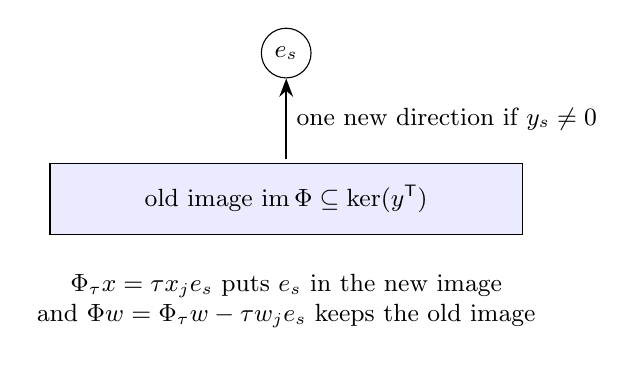
\begin{tikzpicture}[>=Stealth,every node/.style={font=\small}]
\fill[blue!8] (0,0) rectangle (6,.9);
\draw (0,0) rectangle (6,.9);
\node at (3,.45) {old image $\operatorname{im}\Phi\subseteq\ker(y^{\mathsf T})$};
\node[draw,circle,inner sep=3pt] (e) at (3,2.3) {$e_s$};
\draw[->,thick] (3,.95)--node[right] {one new direction if $y_s\ne0$} (e);
\node[align=center] at (3,-.85) {$\Phi_\tau x=\tau x_j e_s$ puts $e_s$ in the new image\\and $\Phi w=\Phi_\tau w-\tau w_j e_s$ keeps the old image};
\end{tikzpicture}

\caption{An image-space schematic for the rank lemma. The rectangle represents a subspace, not a numerical matrix. If both kernel coordinates were nonzero, one allowed perturbation would strictly increase the image dimension.}
\end{figure}

\begin{lemma}[Kernels at maximum support rank]\label{lem:kernel-support}
Let $T\subseteq I\times J$, where $I$ and $J$ are finite.  Suppose that
$\Phi:\R^J\to\R^I$ has maximum rank among all real matrices supported on $T$.
Then, for every $x\in\ker \Phi$, every $y\in\ker \Phi^{\mathsf T}$, and every
$(s,j)\in T$, one has $x_jy_s=0$.
\end{lemma}

\begin{proof}
Suppose instead that $x_jy_s\ne0$.  For a nonzero real $\tau$, the matrix
$\Phi_\tau=\Phi+\tau e_s e_j^{\mathsf T}$ is still supported on $T$, and
\[
 \Phi_\tau x=\tau x_j e_s.
\]
Thus $e_s\in\im \Phi_\tau$.  Moreover, for every $w\in\R^J$,
\[
 \Phi w=\Phi_\tau w-\tau w_j e_s\in\im \Phi_\tau,
\]
so the entire old image $\im \Phi$ is contained in $\im \Phi_\tau$.
On the other hand, $y$ annihilates $\im \Phi$ and $y_s\ne0$, so
$e_s\notin\im \Phi$.  Therefore $\rank \Phi_\tau>\rank \Phi$, a contradiction.
\end{proof}


\paragraph{Proof itinerary.}
The proof has seven explicit goals, in the order used below:
\begin{enumerate}[label=\arabic*.]
\item A small cover of an augmented graph gives the required pruning.
\item A normalized maximum matching splits into $k+\ell+t$ edges, with both coverage parts maximum.
\item Four linear maps satisfy $NL=AB$.
\item Three rank conditions imply $k+\ell+t\le |Z|+|H|$.
\item One coefficient assignment supplies all the needed ranks and coverage bases.
\item Kernel restrictions and normalized lifts supply $k$ independent vectors in $\ker A$.
\item Alternating paths turn the matching bound into the cover from Goal~1.
\end{enumerate}
Goals 4--6 are the algebraic heart. Goal~1 explains the budget we need,
and Goal~7 converts the algebra back into a deletion rule.

\begin{proof}[Proof of Lemma~\ref{lem:pruning}]
If there are no conflicts, retain every member; then $Z=H=\varnothing$
and the assertion is immediate.  In what follows, all vector spaces have
their usual coordinate bases.  Empty minors have determinant $1$, so the
rank arguments also apply when a matching or an index set is empty.

\paragraph{Claim 1: a cover of size $|Z|+|H|$ suffices.}
Form a bipartite graph $\Gamma$ with parts
\[
 \mathcal V_L=\mathcal R\sqcup Z_L,
 \qquad
 \mathcal V_R=\mathcal C\sqcup Z_R,
\]
where $Z_L$ and $Z_R$ are separate copies of $Z$, disjoint also from the
two original families.  Join conflicting original members.  Also join
each original member to the opposite copy of every point of $Z$ that it
covers.  There are no edges between $Z_L$ and $Z_R$.
Figure~\ref{fig:pruning} displays the three edges forced by one conflict.

\begin{figure}[!ht]
 \centering
 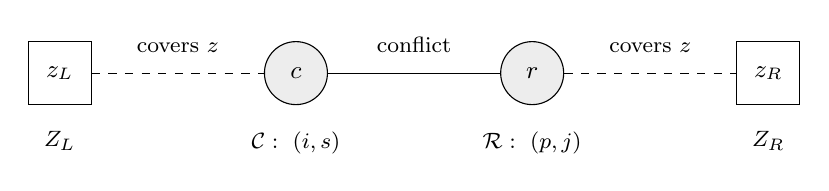
\begin{tikzpicture}[
  every node/.style={font=\small},
  original/.style={circle,draw,fill=black!7,minimum size=8mm,inner sep=1pt},
  copy/.style={rectangle,draw,minimum size=8mm,inner sep=3pt},
  edge label/.style={font=\footnotesize,above=4pt},
  family label/.style={font=\footnotesize,below=6pt}
]
 \node[copy] (zl) at (0,0) {$z_L$};
 \node[original] (c) at (3,0) {$c$};
 \node[original] (r) at (6,0) {$r$};
 \node[copy] (zr) at (9,0) {$z_R$};
 \draw[dashed] (zl) -- node[edge label] {covers $z$} (c);
 \draw (c) -- node[edge label] {conflict} (r);
 \draw[dashed] (r) -- node[edge label] {covers $z$} (zr);
 \node[family label] at (zl.south) {$Z_L$};
 \node[family label] at (c.south) {$\mathcal C:\ (i,s)$};
 \node[family label] at (r.south) {$\mathcal R:\ (p,j)$};
 \node[family label] at (zr.south) {$Z_R$};
\end{tikzpicture}

 \caption{A conflict between $r=(p,j)$ and $c=(i,s)$ forces this path,
 where $z=(i,j)\in Z$.  The copies $z_L$ and $z_R$ are distinct vertices.
 The vertices alternate between the two sides of the bipartition.
 Different conflicts can share vertices and edges; the full augmented
 graph need not be a disjoint union of such paths.}
 \label{fig:pruning}
\end{figure}

An initially conflict-free member is isolated in $\Gamma$.
Indeed, if $(p,j)\in\mathcal R$ covered $(i,j)\in Z$, an original
conflict witnessing $(i,j)\in Z$ would supply a member
$(i,s)\in\mathcal C$ with $s\to j$.  This member would conflict with
$(p,j)$.  The same argument with the sides exchanged applies to
$\mathcal C$.

It suffices to find a vertex cover $K$ of $\Gamma$ of size at most
$\abs Z+\abs H$, omitting isolated vertices.  Delete precisely its
original members.  No conflict then survives.  If $q$ points of $Z$ are
uncovered by the surviving members, each of the other $\abs Z-q$ points
has a surviving member adjacent to one of its two copies.  That copy
must lie in $K$.  Distinct points require distinct new vertices, whence
\begin{equation}\label{eq:cover-charge}
 \abs{K\cap(\mathcal R\sqcup\mathcal C)}
 \leq \abs K-(\abs Z-q)\leq\abs H+q.
\end{equation}
Thus the cover gives exactly~\eqref{eq:pruning-bound} and retains every
initially conflict-free member.

\paragraph{Claim 2: the coverage matchings can both be made maximum.}
We will obtain this cover by proving that a maximum matching in $\Gamma$
has size at most $\abs Z+\abs H$ and then giving the usual alternating-path
construction of the cover.  Choose a maximum matching $\mathcal M$ with
the fewest edges between original members.  Write $k$ for the number of
these edges, and let $\alpha$ and $\beta$ be its edges in
$\mathcal R\times Z_R$ and $Z_L\times\mathcal C$, respectively.  Put
\[
 \ell=\abs\alpha,\qquad t=\abs\beta,
 \qquad\abs{\mathcal M}=k+\ell+t.
\]

Each of $\alpha$ and $\beta$ is a maximum matching in its own subgraph.
For example, if the $\mathcal R$--$Z_R$ subgraph had a larger matching,
its symmetric difference with $\alpha$ would contain an
$\alpha$-augmenting path, starting at an $\alpha$-unmatched member of
$\mathcal R$ and ending at an $\alpha$-unmatched vertex of $Z_R$.
The latter vertex is unmatched in $\mathcal M$, and every internal vertex
of the path is matched by $\alpha$.  If the starting member is unmatched
in $\mathcal M$, augmenting gives a larger matching in $\Gamma$.
Otherwise it lies on an original--original edge of $\mathcal M$;
remove that edge and augment along the path.  This preserves the total
size and reduces $k$.  Both conclusions contradict the choice of
$\mathcal M$.  The proof for $\beta$ is identical with the sides
exchanged.  Denote by $R_\alpha\subseteq\mathcal R$ and
$C_\beta\subseteq\mathcal C$ the original vertices matched by these
two matchings.

\paragraph{Claim 3: the four maps commute, $NL=AB$.}
To bound $k+\ell+t$, we encode the two maximum matchings by matrix ranks.
For each arrow $x\to y$, introduce independent variables $a_{xy}$ and
$b_{xy}$, with the two arrays independent of one another.  Set both
entries to zero when $x\not\to y$.  We shall choose real values for all
the variables shortly.  For any real assignment, define four maps by
\[
 \begin{array}{ccc}
 \R^H&\xleftarrow{\ B\ }&\R^{\mathcal R}\\[3pt]
 {\scriptstyle A}\big\downarrow&&\big\downarrow{\scriptstyle L}\\[3pt]
 \R^{\mathcal C}&\xleftarrow{\ N\ }&\R^Z
 \end{array}
\]
with entries
\begin{equation}\label{eq:pruning-maps}
 \begin{aligned}
 L_{(i,j),(p,j)}&=a_{pi},&
 N_{(i,s),(i,j)}&=b_{sj},\\
 B_{(p,s),(p,j)}&=b_{sj},&
 A_{(i,s),(p,s)}&=a_{pi}.
 \end{aligned}
\end{equation}
The row and column indices in each formula range over its indicated
coordinate sets, and every entry not of a listed form is zero.
The maps $L,A$ change the first coordinate forward along $p\to i$;
$N,B$ change the second coordinate backward from $j$ to $s$ along $s\to j$.
For a conflict, the two routes from $(p,j)$ to $(i,s)$ change the
coordinates in opposite orders, through $(i,j)\in Z$ or $(p,s)\in H$.
For a fixed column $(p,j)\in\mathcal R$ and row
$(i,s)\in\mathcal C$, the only possible intermediate index in $NL$ is
$(i,j)$, and the only possible one in $AB$ is $(p,s)$.  If the two
endpoints conflict, these indices belong to $Z$ and $H$, respectively,
and both products have entry $a_{pi}b_{sj}$.  If they do not conflict,
at least one factor is zero in both products.  Hence
\begin{equation}\label{eq:pruning-commute}
 NL=AB.
\end{equation}


\begin{figure}[ht]\centering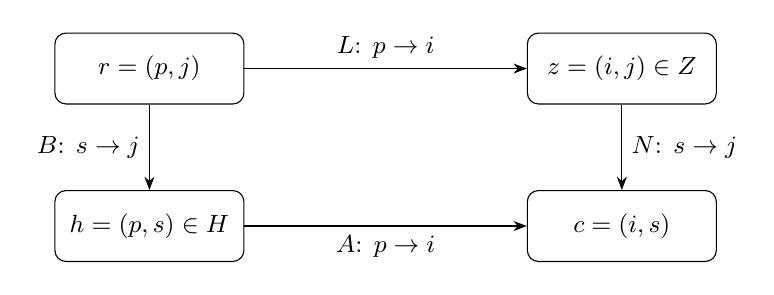
\begin{tikzpicture}[>=Stealth, every node/.style={font=\small}, v/.style={draw,rounded corners,minimum width=24mm,minimum height=9mm}]
\node[v] (r) at (0,0) {$r=(p,j)$};
\node[v] (z) at (6,0) {$z=(i,j)\in Z$};
\node[v] (h) at (0,-2) {$h=(p,s)\in H$};
\node[v] (c) at (6,-2) {$c=(i,s)$};
\draw[->] (r)--node[above] {$L$: $p\to i$} (z);
\draw[->] (r)--node[left] {$B$: $s\to j$} (h);
\draw[->] (z)--node[right] {$N$: $s\to j$} (c);
\draw[->] (h)--node[below] {$A$: $p\to i$} (c);
\end{tikzpicture}

\caption{One conflict and its two intermediate corners. The rows are $p,i$ and the columns are $s,j$, as in the coordinate grid. The vertical maps follow $p\to i$; the horizontal maps run backward along $s\to j$. The two products have the same coefficient $a_{pi}b_{sj}$, yielding $NL=AB$. The two paths from $r$ to $c$ are the two factorizations. In contrast, the set operator $F_2$ follows the second-coordinate relation forward.}
\end{figure}

\paragraph{Claim 4: three rank conditions imply the matching bound.}
We seek an assignment for which
\[
 \rank L=\ell,\qquad \rank N=t,\qquad \dim\ker A\geq k.
\]
These three conditions give the desired matching bound. Indeed,
rank--nullity and $NL=AB$ would give
\begin{align}
 \abs H
 &=\dim\ker A+\rank A\notag\\
 &\geq k+\rank A
 \geq k+\rank(NL)\notag\\
 &\geq k+\ell+t-\abs Z.
 \label{eq:pruning-rank-bound}
\end{align}
The last step is Sylvester's rank inequality. Here is its short proof, obtained by restricting $N$ to $\im L$:
\[
 \rank(NL)
 =\dim\im L-\dim(\im L\cap\ker N)
 \geq\ell-(\abs Z-t).
\]
The first two rank conditions will come from $\alpha$ and $\beta$.
For the third, we will lift the $k$ original left endpoints to vectors
$u^r\in\ker L$ and show that their images $Bu^r$ are independent.
The identity $AB=NL$ places these images in $\ker A$.

\paragraph{Claim 5: one assignment supplies all ranks and coverage bases.}
Our choice of coefficients uses the correspondence between generic matrix
rank and maximum matching size~\cite[Section~5, Theorem~1]{Edmonds1967}.
We apply the determinant argument within coordinate blocks and verify that
all required minors can be nonzero at the same assignment.
We choose the coefficients so that $\rank L=\ell$, with its
$R_\alpha$ columns a basis of $\im L$, and
$\rank N^{\mathsf T}=t$, with its $C_\beta$ columns a basis of
$\im N^{\mathsf T}$.  To justify this choice, a nonzero minor of $L$
requires a matching between its column and row indices: a nonzero term
in its determinant supplies the matching.  Since $\alpha$ is maximum,
$\rank L\leq\ell$ for every coefficient assignment.  The square minor
using precisely the endpoints of $\alpha$ is, up to row and column
ordering, block diagonal by the second coordinate $j$.  In each block
all allowed entries are distinct variables $a_{pi}$.  The matching
gives a determinant monomial that cannot cancel, because different
permutations use different sets of these variables.  Each block
determinant is therefore a nonzero polynomial, and so is their product.
Variables may occur in more than one block, but a product of nonzero
polynomials remains nonzero.  This proves the required independence
when that minor does not vanish.  For $N^{\mathsf T}$ the same argument
uses blocks with the first coordinate $i$ fixed and distinct variables
$b_{sj}$ within each block.

One additional finite collection of rank conditions will be needed.
For every arrow $p\to i$, define
\[
 J_p=\{j:(p,j)\in\mathcal R\},\qquad
 S_i=\{s:(i,s)\in\mathcal C\},\qquad
 \Phi^{p,i}=(b_{sj})_{s\in S_i,\ j\in J_p}.
\]
We require $\Phi^{p,i}$ to have maximum rank among all matrices supported
on
\[
 T^{p,i}=\{(s,j)\in S_i\times J_p:s\to j\}.
\]
These matrices will let Lemma~\ref{lem:kernel-support} compare restrictions
of vectors in $\ker B$ and $\ker N^{\mathsf T}$.
The allowed entries of each individual $\Phi^{p,i}$ are independent
variables.  A minor attaining its maximum possible rank at some
assignment is therefore a nonzero polynomial in the $b$ variables.
Choose one such minor for each arrow, taking the empty minor when the
maximum rank is zero.  Multiply these finitely many polynomials with
the two matching minors just described.  The product is nonzero in the
polynomial ring generated by all $a$ and $b$ variables, even though
variables are shared between different matrices.  A nonzero real
polynomial is nonzero at some real assignment, as follows by induction
on its number of variables.  Fix such an assignment once and for all.
It gives these support ranks and the two basis properties simultaneously.


\paragraph{Why shared coefficients cause no problem.}
We do not choose a different assignment for each matrix. For each desired
rank condition choose a minor that is a nonzero polynomial. Their finite
product is nonzero even if variables recur in different factors. Over the
infinite field $\mathbb R$, some assignment makes the product nonzero.
All the chosen conditions then hold at that one assignment. Later,
perturbing a single auxiliary matrix is only a contradiction argument for
its maximum rank; it does not change the fixed assignment of the square.

\paragraph{Claim 6: normalized lifts give $\dim\ker A\ge k$.}
For every edge $(r,c)$ of $\mathcal M$ between original members, the
basis properties now give vectors
\begin{equation}\label{eq:pruning-lifts}
 \begin{aligned}
 u^r&=e_r+\sum_{a\in R_\alpha}\lambda_a^r e_a
                 \in\ker L,\\
 v^c&=e_c+\sum_{b\in C_\beta}\mu_b^c e_b
                 \in\ker N^{\mathsf T}.
 \end{aligned}
\end{equation}
The original--original endpoints are disjoint from $R_\alpha$ and
$C_\beta$, respectively.  In particular, the $u^r$ restrict to distinct
unit vectors on the $k$ original left endpoints, and $v^c_c=1$.

\paragraph{6a: restrict the full equations to the auxiliary matrices.}
We need one independent vector in $\ker A$ for each of the $k$ remaining
matched edges. The left lifts already give candidates: $u^r\in\ker L$
implies $ABu^r=NLu^r=0$. Only independence of the $Bu^r$ is missing.
It will follow if every vector in $\ker B$ vanishes at the distinguished
left endpoints. The right lifts will act as probes: $v^c_c=1$ turns a
zero product $u_rv^c_c=0$ into $u_r=0$.
First we prove the product statement for arbitrary kernel vectors at the
fixed coefficient assignment:
\begin{equation}\label{eq:conflict-kernel}
 u_{pj}v_{is}=0
 \quad\text{for every conflict }((p,j),(i,s)),
 \quad u\in\ker B,\quad v\in\ker N^{\mathsf T}.
\end{equation}
Here the assertion quantifies over \emph{all} vectors in the two kernels.

To prove it, fix an arrow $p\to i$.  For $u\in\ker B$, consider the
vector $(u_{pj})_{j\in J_p}$.  If a row $s\in S_i$ of $\Phi^{p,i}$ has
an allowed entry, choose $j\in J_p$ with $s\to j$.  Then
$(p,j)$ and $(i,s)$ conflict, so $(p,s)\in H$.  The complete equation
of $Bu=0$ at this coordinate is
\begin{equation}\label{eq:pruning-row-equation}
 \sum_{j\in J_p}b_{sj}u_{pj}=0.
\end{equation}
If the row has no allowed entry, this equation holds because all its
coefficients are zero.  Thus it holds for every $s\in S_i$, including
rows for which $(p,s)$ is absent from $H$.  Consequently
$(u_{pj})_{j\in J_p}\in\ker \Phi^{p,i}$.

Similarly, let $v\in\ker N^{\mathsf T}$.  If a column $j\in J_p$
of $\Phi^{p,i}$ has an allowed entry, choose $s\in S_i$ with $s\to j$.
The resulting conflict implies $(i,j)\in Z$, and the complete equation
of $N^{\mathsf T}v=0$ at this coordinate is
\begin{equation}\label{eq:pruning-column-equation}
 \sum_{s\in S_i}b_{sj}v_{is}=0.
\end{equation}
Columns with no allowed entries satisfy the same equation
automatically.  Hence $(v_{is})_{s\in S_i}\in\ker(\Phi^{p,i})^{\mathsf T}$.
Since $\Phi^{p,i}$ has maximum rank on its allowed support,
Lemma~\ref{lem:kernel-support} gives $u_{pj}v_{is}=0$ whenever
$s\to j$, proving~\eqref{eq:conflict-kernel}.
The hypothetical single-entry perturbation in that lemma concerns only
$\Phi^{p,i}$; it need not preserve any other rank condition.  The conclusion
holds for every pair of kernel vectors at the fixed, original assignment.

\paragraph{6b: use the right lifts to distinguish the left images.}
For each original--original matched edge $(r,c)$, substitute $v=v^c$
in~\eqref{eq:conflict-kernel}.  Since $v^c_c=1$, every vector in
$\ker B$ vanishes at $r$.  It follows that the vectors $Bu^r$, as $r$
ranges over the $k$ original left endpoints, are linearly independent.
Indeed, a relation
\[
 \sum_r\theta_r Bu^r=0
\]
puts the single vector $u=\sum_r\theta_r u^r$ in $\ker B$.
Its coordinate at each such endpoint $r$ is $u_r=\theta_r$, by
\eqref{eq:pruning-lifts}.  All these coordinates vanish, so every
$\theta_r$ is zero.  Furthermore,
\[
 A(Bu^r)=NLu^r=0
\]
by~\eqref{eq:pruning-commute}. Thus $\dim\ker A\geq k$, establishing
the third rank condition. Equation~\eqref{eq:pruning-rank-bound} now gives
$\abs{\mathcal M}=k+\ell+t\leq\abs Z+\abs H$, as required.

\paragraph{Claim 7: the matching bound gives the cover.}
For completeness, we give the matching-to-cover argument in
K\H{o}nig's theorem~\cite{konig1931}.  Starting at all unmatched vertices
of $\mathcal V_L$, follow edges outside $\mathcal M$ from left to
right and edges in $\mathcal M$ from right to left.  Let $W_L,W_R$
be the reached vertices on the two sides.  No unmatched right vertex
is reached, since an alternating path to one would augment the maximum
matching.  The endpoints of a matched edge are either both reached or
both unreached: a reached right endpoint leads to its mate, and a
matched left endpoint can only have been reached through its mate.
It follows that
\[
 K=(\mathcal V_L\setminus W_L)\cup W_R
\]
covers every edge.  Indeed, an edge from a reached left vertex to an
unreached right vertex could be neither an unmatched edge, which would
be traversed, nor a matched edge, whose endpoints have the same
reachability.  The cover contains exactly one endpoint of each matched
edge and no unmatched vertices.  Hence
$\abs K=\abs{\mathcal M}\leq\abs Z+\abs H$; it also omits isolated
vertices.  Applying~\eqref{eq:cover-charge} to this $K$ proves the lemma.
\end{proof}

\section{The extremal contradiction}\label{sec:incompatibility}

We use Lemma~\ref{lem:pruning} to rule out the graph supplied by
Proposition~\ref{prop:counterexample-reduction}.  The proof converts the strict
subset inequalities into a strict increase of an extremal quantity associated
with two families of ordered pairs.


\paragraph{Why pairs, and why this objective?}
The strict inequality applies to one set at a time. Columns of $P$ and rows
of $Q$ provide many such sets while making their images share one ambient
square. Compatibility makes those images disjoint. Taking complements of
second images then produces a gain of more than $2d$. Pruning can cost
$d+d'$, so adding $d'$ to the new objective exactly pays for its output cost.
This explains the choice $|P|+|Q|+d$ before any algebra is performed.
\paragraph{Why the coefficient of uncovered points is one.}
Suppose instead that the objective were $M+\lambda d$. The same gain and
pruning estimates would only give a new objective strictly greater than
$M+d+(\lambda-1)d'$. Relative to the old $M+\lambda d$, its guaranteed
improvement would be strictly greater than $(\lambda-1)(d'-d)$. We have no
comparison between $d$ and $d'$. Choosing $\lambda=1$ removes both unknown
terms and makes the strict improvement automatic.

\paragraph{A numerical budget trace.}
To see the cancellation with numbers, suppose $M=10$, $d=2$, and $d'=3$.
The gain estimate would give at least $15$ members before pruning, since
$|\mathcal L|+|\mathcal R|>M+2d=14$. At most $d+d'=5$ are deleted,
leaving at least $10$ members. Adding the new uncovered count gives a new
objective at least $10+3=13$, exceeding the old $10+2=12$.
These are illustrative budget values, not an asserted graph satisfying
the contradictory hypotheses.

\begin{figure}[ht]\centering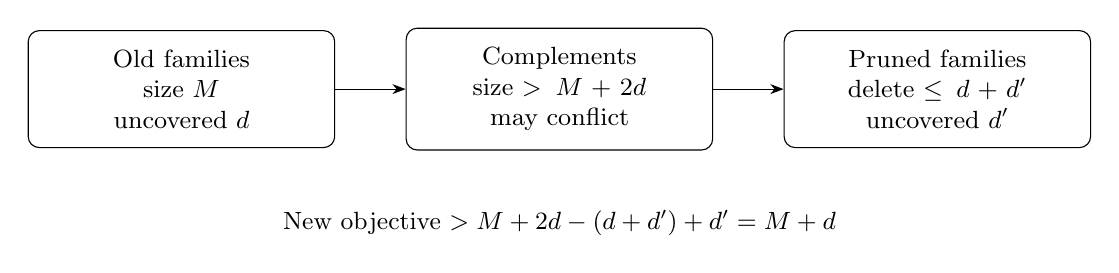
\begin{tikzpicture}[>=Stealth,box/.style={draw,rounded corners,text width=34mm,align=center,inner sep=7pt},every node/.style={font=\small}]
\node[box] (a) at (0,0) {Old families\\size $M$\\uncovered $d$};
\node[box] (b) at (4.8,0) {Complements\\size $>M+2d$\\may conflict};
\node[box] (c) at (9.6,0) {Pruned families\\delete $\le d+d'$\\uncovered $d'$};
\draw[->] (a)--(b);\draw[->] (b)--(c);
\node at (4.8,-1.7) {New objective $>M+2d-(d+d')+d'=M+d$};
\end{tikzpicture}

\caption{The accounting of the contradiction. The second uncovered count $d'$ belongs to the retained families, so it must occur in both the deletion bound and the new objective.}
\end{figure}

\begin{figure}[ht]\centering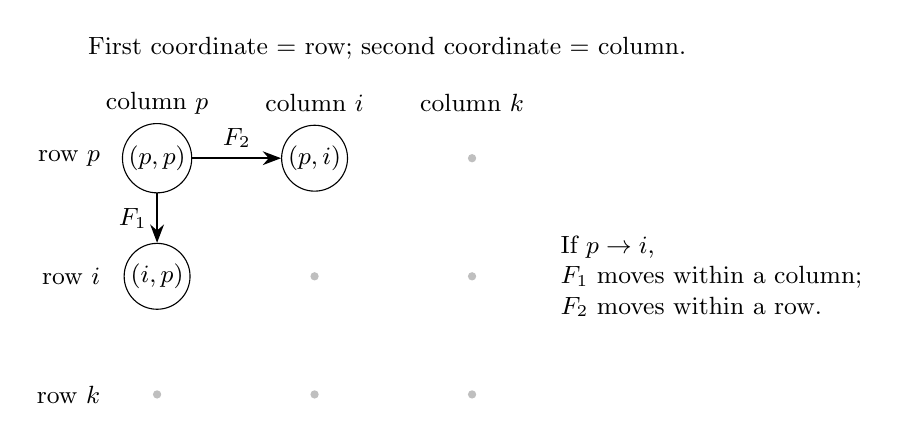
\begin{tikzpicture}[>=Stealth,every node/.style={font=\small},v/.style={circle,draw,minimum size=8mm,inner sep=1pt}]
\node[align=left,anchor=west] at (-1,2.4) {First coordinate = row; second coordinate = column.};
\foreach \x/\j in {0/p,2/i,4/k}{\node at (\x,1.7) {column $\j$};}
\foreach \y/\i in {1/p,-.5/i,-2/k}{\node[anchor=east] at (-.6,\y) {row $\i$};}
\foreach \x in {0,2,4}{\foreach \y in {1,-.5,-2}{\fill[black!25] (\x,\y) circle (1.5pt);}}
\node[v,fill=white] (a) at (0,1) {$(p,p)$};
\node[v,fill=white] (b) at (0,-.5) {$(i,p)$};
\node[v,fill=white] (c) at (2,1) {$(p,i)$};
\draw[->,thick] (a)--node[left] {$F_1$} (b);
\draw[->,thick] (a)--node[above] {$F_2$} (c);
\node[anchor=west,align=left] at (5,-.5) {If $p\to i$,\\$F_1$ moves within a column;\\$F_2$ moves within a row.};
\end{tikzpicture}

\caption{A coordinate convention for set images. The dots are positions in $X\times X$, not vertices of $G$. Image operators use the graph relation on a coordinate; visual adjacency on the grid has no mathematical meaning. The arrow $p\to i$ produces both moves shown.}
\end{figure}
\begin{proposition}\label{prop:no-concavity}
There is no nonempty finite oriented graph $G$ in which every vertex has an
in-neighbor and whose one-step image operator
\[
 F(U)=\{y\in V(G):x\to y\text{ for some }x\in U\}
\]
satisfies
\begin{equation}\label{eq:impossible-concavity}
 \abs{U}+\abs{F^2(U)}<2\abs{F(U)}
 \qquad(\varnothing\ne U\subsetneq V(G)),
\end{equation}
where $F^2=F\circ F$.
\end{proposition}

\begin{proof}
Suppose that such a graph exists, and put $X=V(G)$.  For $S\subseteq X\times X$,
define the two coordinate image operators by
\[
 \begin{aligned}
 F_1S&=\{(i,j): (p,j)\in S\text{ and }p\to i
                     \text{ for some }p\in X\},\\
 F_2S&=\{(i,j): (i,s)\in S\text{ and }s\to j
                     \text{ for some }s\in X\}.
 \end{aligned}
\]
Write $F_1^2=F_1\circ F_1$, $F_2^2=F_2\circ F_2$, and
$\Delta=\{(v,v):v\in X\}$.  Call $P,Q\subseteq X\times X$ \emph{compatible}
if $F_1P\cap F_2Q=\varnothing$.  Equivalently, no left member $(p,j)\in P$
and right member $(i,s)\in Q$ satisfy both $p\to i$ and $s\to j$; this is
precisely the conflict relation in Lemma~\ref{lem:pruning}.

The pair $P=Q=\Delta$ is compatible: a point $(i,j)$ in both images would
require $j\to i$ and $i\to j$, contrary to orientation.  Thus we may choose,
among all compatible pairs with $\Delta\subseteq P\cap Q$, one maximizing
$M+d$, where
\[
 M=\abs{P}+\abs{Q},\qquad
 d=\abs{X}^2-\abs{F_1P}-\abs{F_2Q}.
\]
Such a maximum exists because $X$ is finite.  Compatibility makes $d$ the
number of points outside $F_1P\cup F_2Q$.  Including these uncovered points
in the objective lets the points left uncovered by pruning offset the
corresponding part of the deletion cost.

Every column $P_j=\{p:(p,j)\in P\}$ is nonempty, since $j\in P_j$.
It is also proper.  Indeed, positive indegrees give $F(X)=X$, so $P_j=X$
would imply $X\times\{j\}\subseteq F_1P$.  Choose an in-neighbor $w$ of
$j$.  Then $(w,j)\in F_2\Delta\subseteq F_2Q$, contradicting compatibility.
Likewise every row $Q_i=\{s:(i,s)\in Q\}$ contains $i$.  If $Q_i=X$,
then $\{i\}\times X\subseteq F_2Q$; choosing $w\to i$ gives
$(i,w)\in F_1\Delta\subseteq F_1P$, again a contradiction.
We can therefore sum~\eqref{eq:impossible-concavity} over the columns of $P$
and over the rows of $Q$ to obtain
\begin{equation}\label{eq:strict-fiber-sums}
 \abs{P}+\abs{F_1^2P}<2\abs{F_1P},\qquad
 \abs{Q}+\abs{F_2^2Q}<2\abs{F_2Q}.
\end{equation}

Define new left and right families by taking complements in $X\times X$:
\[
 \mathcal R=(X\times X)\setminus F_2^2Q,
 \qquad
 \mathcal C=(X\times X)\setminus F_1^2P.
\]
The two strict inequalities in~\eqref{eq:strict-fiber-sums} give
\begin{equation}\label{eq:complement-gain}
 \begin{aligned}
 \abs{\mathcal R}+\abs{\mathcal C}
 &=2\abs{X}^2-\abs{F_2^2Q}-\abs{F_1^2P}\\
 &>2\abs{X}^2+M-2\bigl(\abs{F_1P}+\abs{F_2Q}\bigr)
 =M+2d.
 \end{aligned}
\end{equation}
These families need not be compatible.  We will apply the pruning lemma,
first verifying that the diagonal survives and then bounding the cost.


\paragraph{Two diagonal checks, with different purposes.}
First show membership: the diagonal belongs to the prospective families.
Then show isolation: these diagonal members have no conflicts there.
Membership alone would not make pruning preserve them. Isolation invokes
the preservation clause of the pruning lemma. This is what makes the new
pair admissible for the very same extremal problem.

Both families contain $\Delta$.  If $(v,v)\in F_2^2Q$, there is an $s\to v$
with $(v,s)\in F_2Q$.  But $(s,s)\in P$ gives $(v,s)\in F_1P$, a
contradiction.  If $(v,v)\in F_1^2P$, there is a $p\to v$ with
$(p,v)\in F_1P$.  Now $(p,p)\in Q$ gives $(p,v)\in F_2Q$, the same
contradiction.

Moreover, each diagonal member is conflict-free in the new families.
A conflict between the left member $(v,v)$ and a right member
$(i,s)\in\mathcal C$ would give the path $s\to v\to i$.
Starting at $(s,s)\in P$ and expanding its first coordinate twice would
then put $(i,s)$ in $F_1^2P$, contrary to its membership in $\mathcal C$.
A conflict between a left member $(p,j)\in\mathcal R$ and the right member
$(v,v)$ would give $p\to v\to j$.  Expanding the second coordinate of
$(p,p)\in Q$ twice would put $(p,j)$ in $F_2^2Q$, again a contradiction.
The preservation clause of Lemma~\ref{lem:pruning} thus applies to every
diagonal member on both sides.

Let $H,Z\subseteq X\times X$ be the sets associated with
$\mathcal R,\mathcal C$ in that lemma.  Thus each conflict
\[
 (p,j)\in\mathcal R,\quad (i,s)\in\mathcal C,\quad
 p\to i,\quad s\to j
\]
contributes $(p,s)$ to $H$ and $(i,j)$ to $Z$.
We claim that
\begin{equation}\label{eq:old-uncovered-bound}
 H\subseteq (X\times X)\setminus(F_1P\cup F_2Q),
 \qquad\text{and hence}\qquad \abs{H}\le d.
\end{equation}
To see this, fix such a conflict.  If $(p,s)\in F_1P$, choose
$(u,s)\in P$ with $u\to p$.  The path $u\to p\to i$ then puts
$(i,s)$ in $F_1^2P$, contrary to $(i,s)\in\mathcal C$.
If $(p,s)\in F_2Q$, choose $(p,t)\in Q$ with $t\to s$.
The path $t\to s\to j$ puts $(p,j)$ in $F_2^2Q$, contrary to
$(p,j)\in\mathcal R$.  This proves~\eqref{eq:old-uncovered-bound}.

Apply Lemma~\ref{lem:pruning} to obtain conflict-free families
$P'\subseteq\mathcal R$ and $Q'\subseteq\mathcal C$.
They still contain $\Delta$, and their lack of conflicts means
$F_1P'\cap F_2Q'=\varnothing$.  Set
\[
 d'=\abs{X}^2-\abs{F_1P'}-\abs{F_2Q'}.
\]
A point is covered by a kept left member exactly when it belongs to
$F_1P'$, and by a kept right member exactly when it belongs to $F_2Q'$.
Consequently at most $d'$ points of $Z$ are uncovered after pruning.
By Lemma~\ref{lem:pruning} and~\eqref{eq:old-uncovered-bound}, at most $d+d'$ members
were deleted, counting the two sides separately.  Using
\eqref{eq:complement-gain}, we conclude that
\[
 \begin{aligned}
 \abs{P'}+\abs{Q'}+d'
 &\ge \abs{\mathcal R}+\abs{\mathcal C}-(d+d')+d'\\
 &>M+2d-(d+d')+d'=M+d.
 \end{aligned}
\]
This contradicts the choice of $P,Q$ and proves the proposition.
\end{proof}

\begin{proof}[Proof of Theorem~\ref{thm:main}]
If the theorem were false, Proposition~\ref{prop:counterexample-reduction}
would produce a nonempty finite oriented graph with positive indegrees
satisfying~\eqref{eq:impossible-concavity} for every nonempty proper vertex
set.  Proposition~\ref{prop:no-concavity} rules out such a graph.
\end{proof}

\section{Weighted consequences}\label{sec:weighted-consequences}

The following corollary applies Theorem~\ref{thm:main} through Seacrest's
established equivalences of the corresponding assertions over all nonempty
finite oriented graphs~\cite{Seacrest2015}.  The equivalences themselves are
not new here.

\begin{corollary}[Weighted second-neighborhood forms]\label{cor:weighted-forms}
Let \(D\) be a nonempty finite oriented graph, and write \(\operatorname{Arc}(D)\) for its
arc set.  For a vertex weighting \(\eta:V(D)\to[0,\infty)\), write
\(\eta(S)=\sum_{x\in S}\eta(x)\).  Then the following hold.
\begin{enumerate}[label=\textup{(\roman*)}]
\item For every vertex weighting \(\eta:V(D)\to[0,\infty)\), there is a
vertex \(v\in V(D)\) such that
\[
 \eta(N_1^+(v))\leq\eta(N_2^+(v)).
\]

\item There is a vertex weighting \(\eta:V(D)\to[0,\infty)\) with
\(\sum_{x\in V(D)}\eta(x)=1\) such that
\[
 \eta(N_1^+(v))\leq\eta(N_2^+(v))\qquad\text{for every }v\in V(D).
\]
The entries of this weighting need not all be positive.

\item For every arc weighting \(w:\operatorname{Arc}(D)\to[0,\infty)\), extend the notation
by setting \(w(vs)=0\) when \(vs\notin \operatorname{Arc}(D)\).  For \(v,s\in V(D)\), put
\[
 \beta_v^w(s)=\max\Bigl(\{0\}\cup
 \{w(us)-w(vs):u\in V(D),\ v\to u\to s\}\Bigr).
\]
Then there is a vertex \(v\in V(D)\) such that
\[
 \sum_{s\in V(D)}\beta_v^w(s)
 \geq \sum_{u\in N_1^+(v)}w(vu).
\]
The maximum is zero if there is no indicated two-step path.  Such paths
are determined by the arcs of \(D\), so an arc of weight zero is still
present and is not treated as a missing arc.
\end{enumerate}
\end{corollary}

\begin{proof}
Seacrest's Proposition~2 proves that his arc-weighted Conjecture~4 is
equivalent to the unweighted conjecture, so Theorem~\ref{thm:main} gives
\textup{(iii)}.

To obtain \textup{(i)}, set $w(us)=\eta(s)$ on every arc.  For each $v,s$,
\[
 \beta_v^w(s)=
 \begin{cases}
  \eta(s),&s\in N_2^+(v),\\
  0,&s\notin N_2^+(v).
 \end{cases}
\]
Indeed, when $v\to s$, every eligible difference $w(us)-w(vs)$ is zero.
At an exact second out-neighbor, $w(vs)=0$ and the maximum is $\eta(s)$;
no other endpoint contributes.  Thus the two sides of \textup{(iii)}
become $\eta(N_2^+(v))$ and $\eta(N_1^+(v))$.  This is the
specialization noted immediately after Seacrest's Proposition~2.

For \textup{(ii)}, let $M_D$ have entry $1$ at $(v,s)$ when
$s\in N_2^+(v)$, entry $-1$ when $s\in N_1^+(v)$, and zero otherwise.
Reversing all arcs transposes this matrix:
$M_{\overleftarrow D}=M_D^{\mathsf T}$.  Seacrest's Theorem~1 applies
Farkas' lemma to give either a nonzero $\eta\ge0$ with $M_D\eta\ge0$,
or a $\xi\ge0$ with $M_D^{\mathsf T}\xi<0$ at every coordinate.
The latter contradicts \textup{(i)} on $\overleftarrow D$.
Normalize the former weighting to total weight one, proving \textup{(ii)}.
\end{proof}

\begin{remark}[A direct way to understand the vertex-weighted form]
There is also a direct route from the unweighted theorem to \textup{(i)}.
For nonnegative integer weights, replace vertex $x$ by an independent set
of size $\eta(x)$, putting all arcs between blocks prescribed by $D$.
If the total weight is zero the assertion is immediate; otherwise the
new graph is nonempty and oriented. A good clone of $v$ has exactly
$\eta(N_1^+(v))$ first neighbors. Its exact second neighbors lie in the
blocks of $N_2^+(v)$, and so there are at most $\eta(N_2^+(v))$ of them.
Consequently its unweighted inequality gives the desired weighted one.
The containment can be strict when a two-step path in $D$ has a zero-weight
intermediate vertex; only an upper bound is needed. Clear denominators for
rational weights. Finally approximate any nonnegative real weighting by
nonnegative rational weightings. Since $D$ has finitely many vertices,
some witness vertex occurs along an infinite subsequence. Taking limits
in its finite sums proves the real-weight assertion.

The two vertex-weighted forms have different witnesses. In \textup{(i)}
the vertex may depend on an arbitrarily specified weighting. In
\textup{(ii)} the weighting is chosen so that all vertices work at once.
Zero entries can be necessary: in the graph with the sole arc $a\to b$,
requiring both vertices to work forces $\eta(b)=0$, whereas
$\eta(a)=1$, $\eta(b)=0$ is a valid normalized solution.
\end{remark}

\section{Directed-cycle consequences}\label{sec:directed-cycle-consequences}

In an oriented graph with no directed triangle, every exact second
out-neighbor is a non-neighbor.  Combining this observation with
Theorem~\ref{thm:main} gives degree and order bounds.
The first assertion below is the oriented-graph form of Thomass\'e's
non-neighbor statement recorded by
Sullivan~\cite[Conjecture~6.12]{Sullivan2006}.
The consequence using both minimum indegree and minimum outdegree is also
noted in \cite[Section~3]{Sullivan2006}.  The regular case gives the
girth-four lower bound in the Behzad--Chartrand--Wall minimum-order
conjecture~\cite{BehzadChartrandWall1970}, also recorded by
Sullivan~\cite[Section~4]{Sullivan2006}.

\begin{corollary}[Non-neighbors and directed cycles]\label{cor:directed-cycle-consequences}
Let \(D\) be a nonempty finite oriented graph of order \(n\).  For
\(v\in V(D)\), write
\[
 N_1^-(v)=\{u:u\to v\},\qquad
 d^\pm(v)=\abs{N_1^\pm(v)},\qquad
 \delta^\pm(D)=\min_{x\in V(D)}d^\pm(x).
\]
Define the non-neighbors of \(v\), excluding \(v\) itself, by
\[
 \overline N(v)=V(D)\setminus
 \bigl(\{v\}\cup N_1^+(v)\cup N_1^-(v)\bigr).
\]
Then the following hold.
\begin{enumerate}[label=\textup{(\roman*)}]
\item If \(D\) has no directed \(3\)-cycle, then some vertex \(v\) satisfies
\[
 d^+(v)\leq\abs{\overline N(v)},\qquad
 n-1\geq 2d^+(v)+d^-(v).
\]
\item If \(\delta^+(D)\geq n/3\) and \(\delta^-(D)\geq n/3\), then \(D\)
contains a directed \(3\)-cycle.
\item If \(r\geq1\) is an integer, \(d^+(v)=d^-(v)=r\) for every vertex,
and \(D\) has directed girth exactly four, then \(n\geq3r+1\).
\end{enumerate}
Here directed girth is the length of a shortest directed cycle.
\end{corollary}

\begin{proof}
Suppose that \(D\) has no directed \(3\)-cycle.  If \(w\in N_2^+(v)\),
choose a path \(v\to u\to w\).  The exact-distance definition excludes
\(w=v\) and \(w\in N_1^+(v)\).  If \(w\in N_1^-(v)\), the arc \(w\to v\)
would close a directed \(3\)-cycle.  Thus
\(N_2^+(v)\subseteq \overline N(v)\) for every \(v\).  Theorem~\ref{thm:main}
now gives a vertex with
\[
 d^+(v)\leq\abs{N_2^+(v)}\leq\abs{\overline N(v)}.
\]
Since \(D\) is oriented, its first in- and out-neighborhoods are disjoint,
and their cardinalities are the corresponding degrees.  Hence
\[
 n-1=d^+(v)+d^-(v)+\abs{\overline N(v)}
 \geq 2d^+(v)+d^-(v),
\]
proving \textup{(i)}.

Under the hypotheses of \textup{(ii)}, absence of a directed \(3\)-cycle
would therefore give
\[
 n-1\geq2\delta^+(D)+\delta^-(D)\geq n,
\]
a contradiction.  The integer degree thresholds are
\(\delta^\pm(D)\geq\lceil n/3\rceil\), so this includes the endpoint
when \(3\) divides \(n\).  Finally, directed girth four excludes directed
\(3\)-cycles; in the regular case the count in \textup{(i)} becomes
\(n-1\geq3r\), proving \textup{(iii)}.
\end{proof}


\begin{remark}
The order count in \textup{(iii)} only needs triangle-freeness. Thus every
nonempty triangle-free oriented graph with $d^+=d^-=r$ satisfies
$n\ge3r+1$, even without specifying its girth. The directed $4$-cycle
attains equality when $r=1$. The companion Lean checks now verify this
stronger form by combining the DeepSeep4.1 cycle lemmas with the rebuilt
reference main theorem and explicit neighborhood-definition bridges.
\end{remark}

\section{Verification and scope of this exposition}
This exposition is a modified version of the supplied OpenAI preprint,
licensed under Apache 2.0 in the parent repository. The main proof text and
bibliography are derived from that source. The reading guide, explanatory
paragraphs, new figures, presentation, experiments, and Lean development
are additions. Historical attributions and external weighted equivalences
are retained as source attributions; their original papers have not been
independently audited here.

The main proof has three logically separate dependencies:
\begin{enumerate}
\item Minimality supplies a subset deficit, and blowup amplifies its integer
slack. Deletion is always restarted from the original minimal graph.
\item Pruning applies to arbitrary finite relations. Its proof uses real
linear algebra, simultaneous nonvanishing of finitely many minors, and the
matching--cover theorem (whose alternating-path proof is included).
\item The extremal argument uses orientation to make the diagonal pair
compatible, and positive indegrees to ensure its fibers are proper.
\end{enumerate}
The ledger accompanying this document records checks of these interfaces.
Finite experiments are regression checks for definitions and charging;
they do not establish the theorem for arbitrary order. The Lean development proves selected set-image identities, the matrix maximum-support-rank kernel lemma via a rank-one
perturbation, independence of the lifted images under explicit
coordinate hypotheses, the commuting-square rank bound, and the numerical
contradiction. It does not yet formalize the construction of the matching
lifts, the simultaneous generic coefficient assignment, or the
minimal-counterexample reductions. It therefore is not a formal proof of
the whole theorem.

\paragraph{A useful consequence to keep separate from the core.}
The directed-cycle corollaries use only the proved second-neighborhood
assertion and a partition of the vertex set. The weighted forms additionally
use the externally cited equivalences and Farkas alternative. A reader
checking the new pruning argument need not accept those external inputs to
check the unweighted implication. The normalized weighting in the second
weighted form may have zero entries; strict positivity is not asserted.

\section{Historical context from the source}
The following literature summary is retained from the supplied preprint;
it is not an independent survey of the current literature.

The conjecture was recorded by Dean and Latka~\cite{DeanLatka1995}.
A \emph{tournament} is an oriented graph with an arc between every pair of
distinct vertices.  This case, also known as Dean's conjecture, was proved
by Fisher~\cite{Fisher1996} using a probability distribution obtained from
Farkas' lemma.  Havet and Thomass\'e gave a combinatorial proof using
local median orders~\cite{HavetThomasse2000}.  Fidler and
Yuster~\cite{FidlerYuster2007} extended the tournament theorem to
tournaments missing a matching, a star, or a clique.  Ghazal corrected the
star-case proof and treated generalized stars~\cite{Ghazal2012}.
Subsequent advances include a matching together with a
star~\cite{DaraFrancisJacobNarayanan2022} and two
stars~\cite{DaamouchAlMninyGhazal2025}.

Other approaches impose degree conditions or weaken the desired ratio.
Kaneko and Locke established the conjecture for minimum outdegree at most
six~\cite{KanekoLocke2001}; a recent computer-assisted preprint treats
minimum outdegree seven~\cite{SadhukhanSandeepSen2026}.
Chen, Shen and Yuster proved a universal second-to-first neighborhood
ratio of approximately $0.657298$~\cite{ChenShenYuster2003}.
Huang and Peng raise this to approximately $0.715538$ and additionally
report a computational bound of $0.74530$~\cite{HuangPeng2024}.
Botler, Moura and Naia~\cite{BotlerMouraNaia2023}, followed by
Espuny D\'iaz, Gir\~ao, Granet and Kronenberg~\cite{EspunyDiazEtAl2025},
studied every orientation of binomial random graphs; the latter result
covers every fixed edge probability below $1/2$, with probability tending
to one as the order tends to infinity.  Brukhman's recent dense-case
preprint concerns graphs of order $n\leq 2\delta+2$, where $\delta$ is
the minimum outdegree~\cite{Brukhman2026}.

\bibliographystyle{plain}
\bibliography{references}
\end{document}
